%!TEX root = ../report.tex

\section{TCP SYN Cookies}

\subsection{TCP SYN Flood Attack}
During an TCP SYN Flood Attack an attacker sends large amounts of packets with spoofed source addresses to the victim.
This fills up their connection table with half open connections (sequence numbers) which results in legitimate users not being able to establish new TCP connections.
A solution for this are TCP SYN cookies.

\subsection{TCP SYN Cookies}
TCP SYN Cookies are particularly chosen initial sequence numbers $\alpha = h(S,K_{SYN})$ where $K$ is a secret key, $S_{SYN}$ the source address of the SYN packet and $h$ a cryptographic hash function.
On arrival of the ACK message, Bob calculates $\alpha$ again and checks if the ACK number is correct ($\alpha + 1$).
This process is shown in Figure~\ref{fig:tcp_syn_cookies}.
\begin{figure}[h]
  \centering
  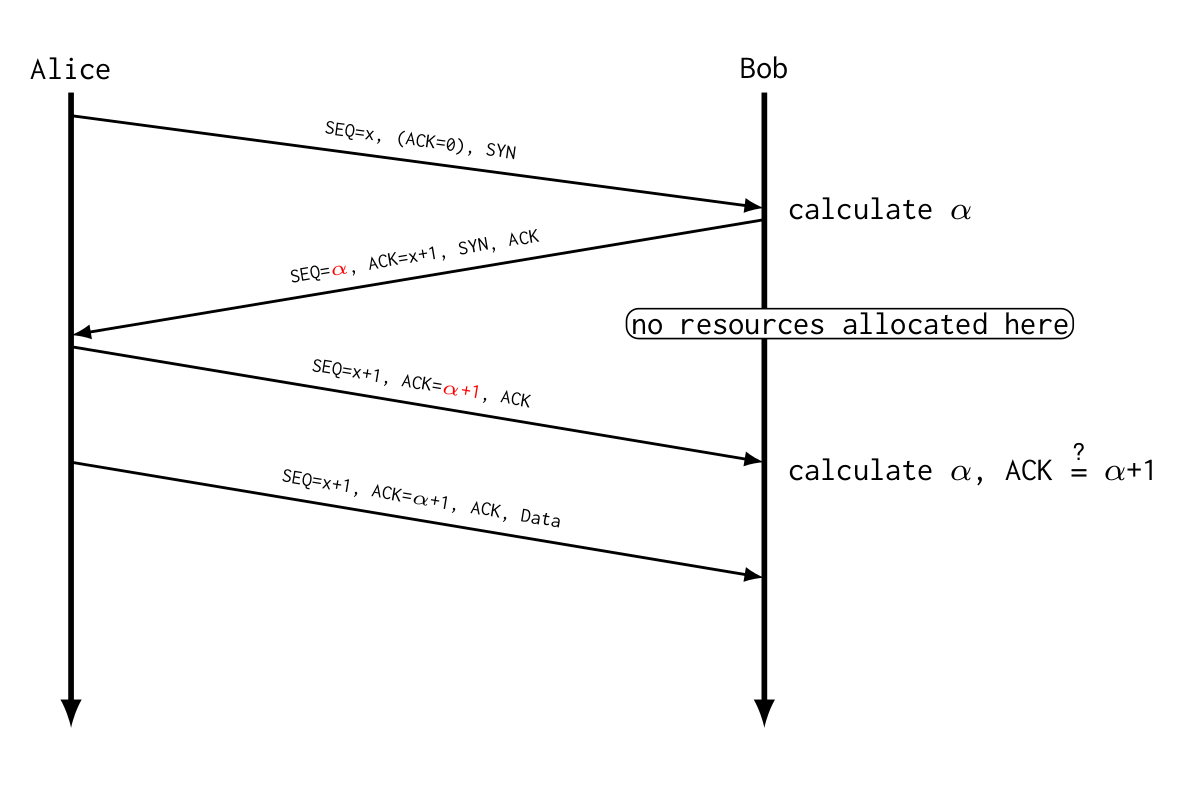
\includegraphics[width=.6\textwidth]{figures/tcp_syn_cookies.png}
  \caption{TCP SYN Cookies}\label{fig:tcp_syn_cookies}
\end{figure}

\begin{minipage}[t]{0.49\textwidth}
  \textbf{Pros}
  \begin{itemize}[topsep=0pt,noitemsep]
    \item No resource allocation after SYN packets
    \item Client does not have to be aware of the server using SYN cookies
    \item No changes in the TCP protocol necessary
  \end{itemize}
\end{minipage}
\begin{minipage}[t]{0.49\textwidth}
  \textbf{Cons}
  \begin{itemize}[topsep=0pt, noitemsep]
    \item Calculating $\alpha$ may be CPU consuming (Linux implementation: CPU local with high cashing efficiency)
    \item TCP options (like large windows size) cannot be negotiated (Linux implementation: window size hacked into cookie, SYN cookies only enabled if a threshold of connections is exceeded)
    \item Efficient implementations might be vulnerable to cryptoanalysis (Linux implementation: SHA used, counter updated every minute)
  \end{itemize}
\end{minipage}
\vspace{20pt}

